\chapter{Laboratorio}
  Para la realización de la actividad practica de laboratorio, se requieren los siguientes materiales/elementos:
  \begin{itemize}
    \item Radio transmisor UHF Alinco DR 430,
    \item Vatimetro de RF Bird modelo 43,
    \item Base magnética para antena,
    \item Irradiantes para la base magnética: $31.7cm$, $17cm$, $16cm$ y $13.5cm$,
    \item Fuente de alimentación $12V$.
  \end{itemize}

  \section{Actividades}
    \begin{enumerate}
      \item \begin{minipage}[t]{\linewidth}
        Verificar los datos del transmisor y vatímetro a fin de evitar daños a los instrumentos. Verificar estado de fuentes de alimentación del transmisor.
        
        \begin{center}
          \includegraphics[width=0.28\textwidth]{img/conexion_inicial.jpeg}
          \captionof{figure}{Conexión inicial del equipamiento.}
          \label{fig:conexion_inicial}
        \end{center}
        \end{minipage}
      \item \begin{minipage}[t]{\linewidth}
        Seleccionar el acoplador para una potencia de 10 W y una frecuencia de 200 a 500 MHz.
        
        \begin{center}
          \includegraphics[width=0.28\textwidth]{img/vatimetro_10w.png}
          \captionof{figure}{Vatímetro configurado para 10W.}
          \label{fig:vatimetro_10w}
        \end{center}
        \end{minipage}
      \item Se posee 4 irradiantes (31.70 cm, 17 cm, 16 cm y 13,5 cm) colocar uno de los irradiantes en la base magnética.
      \item No encender los transmisores antes de hacer las conexiones de los elementos.
      \item \begin{minipage}[t]{\linewidth}
        Conectar mediante cable coaxial el vatímetro entre el transmisor y la antena.
        
        \begin{center}
          \includegraphics[width=0.28\textwidth]{img/Conexion_vatimetro.jpeg}
          \captionof{figure}{Conexión del vatímetro entre transmisor y antena.}
          \label{fig:conexion_vatimetro}
        \end{center}
        \end{minipage}
      \item \begin{minipage}[t]{\linewidth}
        Ajustar la frecuencia de transmisor a: 450 MHz.
        
        \begin{center}
          \includegraphics[width=0.28\textwidth]{img/frecuencia.png}
          \captionof{figure}{Ajuste de frecuencia a 450 MHz.}
          \label{fig:frecuencia}
        \end{center}
        \end{minipage}
      \item Configurar el medidor para medición de potencia incidente como lo indica figura \ref{fig:power_meas.forward}.
        \begin{figure}[!ht]
          \centering
          
\definecolor{c231f20}{RGB}{35,31,32}


\def \globalscale {2.000000}
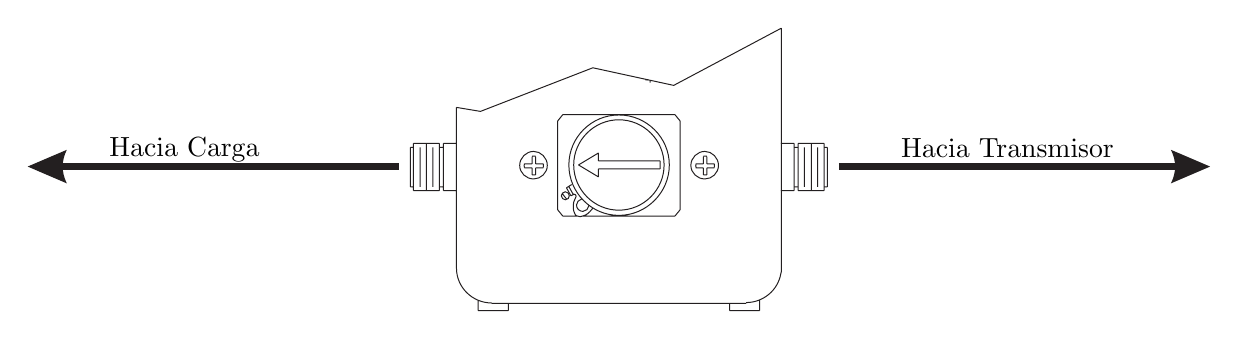
\begin{tikzpicture}[y=1cm, x=1cm, yscale=\globalscale,xscale=\globalscale, every node/.append, inner sep=0pt, outer sep=0pt]
  \begin{scope}[cm={ 0.2646,-0.0,-0.0,0.2646,(-7.9477, 8.3302)}]
    \path[draw=c231f20,line cap=butt,line join=miter,line width=0.0126cm,miter limit=2.613,cm={ 1.3333,-0.0,-0.0,-1.3333,(0.0, -101.4062)}] (30.247, -56.1046) -- (30.679, -56.0326) -- (32.702, -56.8176) -- (34.157, -56.5006) -- (36.094, -57.5306)(31.183, -52.4476) -- (30.636, -52.4476)(30.247, -53.2106).. controls (30.247, -52.8646) and (30.535, -52.5846) .. (30.881, -52.5846)(29.419, -54.6726) -- (29.419, -55.3846)(29.592, -55.3846) -- (29.592, -54.6726)(29.822, -55.3846) -- (29.822, -54.6726)(29.47, -54.6076) -- (29.47, -55.4566)(29.707, -55.4566) -- (29.707, -54.6076)(29.938, -54.6076) -- (29.938, -55.4566)(30.01, -54.6076) -- (30.01, -55.4566)(30.247, -56.1046) -- (30.247, -53.2036)(30.636, -52.6276) -- (30.636, -52.4476)(30.01, -54.6726) -- (29.938, -54.6726)(29.47, -54.6726) -- (29.419, -54.6726)(29.47, -54.6076) -- (29.938, -54.6076)(30.01, -54.6076) -- (30.247, -54.6076)(30.01, -55.3846) -- (29.938, -55.3846)(29.47, -55.3846) -- (29.419, -55.3846)(29.47, -55.4566) -- (29.938, -55.4566)(30.01, -55.4566) -- (30.247, -55.4566)(36.922, -54.6726) -- (36.922, -55.3846)(36.864, -54.6076) -- (36.864, -55.4566)(36.749, -55.3846) -- (36.749, -54.6726)(36.511, -55.3846) -- (36.511, -54.6726)(36.396, -54.6076) -- (36.396, -55.4566)(36.324, -54.6076) -- (36.324, -55.4566)(36.634, -55.4566) -- (36.634, -54.6076)(34.272, -55.8606) -- (34.272, -54.2616)(36.094, -53.1456) -- (36.094, -57.5306)(32.069, -55.8606) -- (32.069, -54.2616)(33.984, -55.0686).. controls (33.984, -55.5146) and (33.617, -55.8816) .. (33.17, -55.8816).. controls (32.724, -55.8816) and (32.357, -55.5146) .. (32.357, -55.0686).. controls (32.357, -54.6216) and (32.724, -54.2546) .. (33.17, -54.2546).. controls (33.617, -54.2546) and (33.984, -54.6216) .. (33.984, -55.0686) -- cycle(34.078, -55.0686).. controls (34.078, -55.5646) and (33.667, -55.9686) .. (33.17, -55.9686).. controls (32.674, -55.9686) and (32.27, -55.5646) .. (32.27, -55.0686).. controls (32.27, -54.5716) and (32.674, -54.1606) .. (33.17, -54.1606).. controls (33.667, -54.1606) and (34.078, -54.5716) .. (34.078, -55.0686) -- cycle(30.881, -52.5766) -- (35.46, -52.5766)(30.881, -52.5766) -- (30.881, -52.5766)(31.183, -52.4476) -- (31.183, -52.5766)(35.46, -52.5916) -- (35.46, -52.5916).. controls (35.77, -52.5916) and (36.036, -52.8146) .. (36.086, -53.1166)(35.705, -52.6276) -- (35.705, -52.4476)(35.165, -52.4476) -- (35.165, -52.5766)(35.165, -52.4476) -- (35.705, -52.4476)(36.086, -53.1166).. controls (36.094, -53.1246) and (36.094, -53.1386) .. (36.094, -53.1456)(32.234, -54.4486) -- (32.148, -54.5566)(32.278, -54.5136).. controls (32.278, -54.5496) and (32.249, -54.5856) .. (32.206, -54.5856).. controls (32.17, -54.5856) and (32.134, -54.5496) .. (32.134, -54.5136).. controls (32.134, -54.4776) and (32.17, -54.4416) .. (32.206, -54.4416).. controls (32.249, -54.4416) and (32.278, -54.4776) .. (32.278, -54.5136) -- cycle(32.4, -54.4996).. controls (32.386, -54.4706) and (32.371, -54.4346) .. (32.357, -54.3986).. controls (32.35, -54.3696) and (32.35, -54.3336) .. (32.35, -54.2976).. controls (32.35, -54.2616) and (32.357, -54.2326) .. (32.371, -54.2046).. controls (32.378, -54.1826) and (32.393, -54.1606) .. (32.407, -54.1536).. controls (32.429, -54.1466) and (32.45, -54.1396) .. (32.465, -54.1396).. controls (32.472, -54.1396) and (32.472, -54.1396) .. (32.479, -54.1396).. controls (32.508, -54.1466) and (32.544, -54.1536) .. (32.573, -54.1686).. controls (32.602, -54.1826) and (32.623, -54.2046) .. (32.652, -54.2326).. controls (32.666, -54.2476) and (32.681, -54.2616) .. (32.695, -54.2836)(32.501, -54.4566).. controls (32.45, -54.4416) and (32.407, -54.3986) .. (32.407, -54.3486).. controls (32.407, -54.2836) and (32.458, -54.2326) .. (32.522, -54.2326).. controls (32.58, -54.2326) and (32.623, -54.2836) .. (32.63, -54.3336)(34.178, -54.1466) -- (32.515, -54.1466)(32.069, -54.2616) -- (32.162, -54.1466)(32.422, -54.1466) -- (32.162, -54.1466)(34.178, -54.1466) -- (34.272, -54.2616)(33.912, -54.9966) -- (32.803, -54.9966)(33.912, -55.1406) -- (32.803, -55.1406)(31.673, -55.0176) -- (31.673, -54.8886);



    \path[draw=c231f20,line cap=butt,line join=miter,line width=0.0126cm,miter limit=2.613,cm={ 1.3333,-0.0,-0.0,-1.3333,(0.0, -101.4062)}] (31.608, -55.0176) -- (31.608, -54.8886)(31.882, -55.0606).. controls (31.882, -55.1976) and (31.766, -55.3126) .. (31.637, -55.3126).. controls (31.5, -55.3126) and (31.385, -55.1976) .. (31.385, -55.0606).. controls (31.385, -54.9246) and (31.5, -54.8166) .. (31.637, -54.8166).. controls (31.766, -54.8166) and (31.882, -54.9246) .. (31.882, -55.0606) -- cycle(31.608, -54.8886).. controls (31.615, -54.8886) and (31.63, -54.8886) .. (31.637, -54.8886).. controls (31.651, -54.8886) and (31.658, -54.8886) .. (31.673, -54.8886)(32.27, -54.6796) -- (32.35, -54.5356)(32.321, -54.7156) -- (32.227, -54.6576)(32.4, -54.4996) -- (32.4, -54.5066).. controls (32.4, -54.5286) and (32.386, -54.5426) .. (32.357, -54.5426).. controls (32.357, -54.5426) and (32.35, -54.5426) .. (32.342, -54.5426)(32.35, -54.5356) -- (32.306, -54.5136)(32.227, -54.6576) -- (32.306, -54.5136)(31.673, -55.0176) -- (31.81, -55.0176)(31.673, -55.0896) -- (31.81, -55.0896)(31.673, -55.2266).. controls (31.666, -55.2266) and (31.651, -55.2266) .. (31.637, -55.2266).. controls (31.63, -55.2266) and (31.615, -55.2266) .. (31.608, -55.2266)(31.673, -55.2196) -- (31.673, -55.0896)(31.608, -55.2196) -- (31.608, -55.0896)(31.471, -55.0896).. controls (31.464, -55.0756) and (31.464, -55.0686) .. (31.464, -55.0536).. controls (31.464, -55.0466) and (31.464, -55.0396) .. (31.471, -55.0246)(31.471, -55.0896) -- (31.608, -55.0896)(31.471, -55.0176) -- (31.608, -55.0176)(33.912, -54.9966) -- (33.912, -55.1406)(31.81, -55.0246).. controls (31.81, -55.0326) and (31.81, -55.0466) .. (31.81, -55.0536).. controls (31.81, -55.0686) and (31.81, -55.0826) .. (31.81, -55.0896)(32.803, -55.1406) -- (32.803, -55.2846)(32.443, -55.0686) -- (32.803, -55.2846)(32.803, -54.8526) -- (32.803, -54.9966)(32.803, -54.8526) -- (32.443, -55.0686)(34.754, -55.0176) -- (34.754, -54.8886)(34.69, -55.0176) -- (34.69, -54.8886)(34.963, -55.0606).. controls (34.963, -55.1976) and (34.848, -55.3126) .. (34.718, -55.3126).. controls (34.582, -55.3126) and (34.466, -55.1976) .. (34.466, -55.0606).. controls (34.466, -54.9246) and (34.582, -54.8166) .. (34.718, -54.8166).. controls (34.848, -54.8166) and (34.963, -54.9246) .. (34.963, -55.0606) -- cycle(34.69, -54.8886).. controls (34.704, -54.8886) and (34.718, -54.8886) .. (34.726, -54.8886).. controls (34.733, -54.8886) and (34.747, -54.8886) .. (34.754, -54.8886)(34.891, -55.0246).. controls (34.891, -55.0326) and (34.891, -55.0466) .. (34.891, -55.0536).. controls (34.891, -55.0686) and (34.891, -55.0826) .. (34.891, -55.0896)(34.754, -55.2266).. controls (34.747, -55.2266) and (34.733, -55.2266) .. (34.726, -55.2266).. controls (34.718, -55.2266) and (34.704, -55.2266) .. (34.69, -55.2266)(34.56, -55.0896).. controls (34.553, -55.0756) and (34.553, -55.0686) .. (34.553, -55.0536).. controls (34.553, -55.0466) and (34.553, -55.0396) .. (34.56, -55.0246)(34.553, -55.0896) -- (34.69, -55.0896)(34.553, -55.0176) -- (34.69, -55.0176)(34.754, -55.2196) -- (34.754, -55.0896)(34.69, -55.2196) -- (34.69, -55.0896)(34.754, -55.0176) -- (34.891, -55.0176)(34.754, -55.0896) -- (34.891, -55.0896)(36.864, -54.6726) -- (36.922, -54.6726)(36.324, -54.6726) -- (36.396, -54.6726)(36.864, -54.6076) -- (36.396, -54.6076)(36.324, -54.6076) -- (36.086, -54.6076)(34.178, -55.9756) -- (32.162, -55.9756)(32.162, -55.9756) -- (32.069, -55.8606)(34.272, -55.8606) -- (34.178, -55.9756)(33.732, -56.5946) -- (33.732, -56.5516)(33.646, -56.6016) -- (33.703, -56.6016)(36.864, -55.3846) -- (36.922, -55.3846)(36.324, -55.3846) -- (36.396, -55.3846)(36.864, -55.4566) -- (36.396, -55.4566)(36.324, -55.4566) -- (36.086, -55.4566);



    \path[draw=c231f20,line cap=butt,line join=miter,line width=0.0843cm,miter limit=2.613,cm={ 1.3333,-0.0,-0.0,-1.3333,(0.0, -101.4062)}] (37.13, -55.0396) -- (43.459, -55.0396);



    \path[fill=c231f20,even odd rule,cm={ 1.3333,-0.0,-0.0,-1.3333,(0.0, -101.4062)}] (43.812, -55.0396) -- (43.106, -55.3416).. controls (43.207, -55.1406) and (43.207, -54.9386) .. (43.106, -54.7366) -- (43.812, -55.0396);



    \path[draw=c231f20,line cap=butt,line join=miter,line width=0.0843cm,miter limit=2.613,cm={ 1.3333,-0.0,-0.0,-1.3333,(0.0, -101.4062)}] (29.21, -55.0396) -- (22.882, -55.0396);



    \path[fill=c231f20,even odd rule,cm={ 1.3333,-0.0,-0.0,-1.3333,(0.0, -101.4062)}] (22.529, -55.0396) -- (23.234, -54.7366).. controls (23.134, -54.9386) and (23.134, -55.1406) .. (23.234, -55.3416) -- (22.529, -55.0396);



    \node[anchor=south west] (text31) at (32, -27.9){Hacia Carga};



    \node[anchor=south west] (text1) at (51, -27.8){Hacia Transmisor};



  \end{scope}

\end{tikzpicture}

          \caption{disposición para medición de potencia incidente.}
          \label{fig:power_meas.forward}
        \end{figure}
      \item \begin{minipage}[t]{\linewidth}
        Encender el medidor y el transmisor. Pulsar el botón de transmisión y verificar que el sistema está transmitiendo.
        
        \begin{center}
          \includegraphics[width=0.8\textwidth]{img/Prueba_transm.jpeg}
          \captionof{figure}{Prueba de transmisión del sistema.}
          \label{fig:prueba_transm}
        \end{center}
        \end{minipage}
      \item Realizar la medición pulsando momentáneamente el botón de transmisión.
        \begin{equation*}
          P_i = *W
        \end{equation*}
        \begin{itemize}
          \item p/10 cm \quad Valor de la \( P_i \) (W) = 3.2
          \item p/13,7 cm \quad Valor de la \( P_i \) (W) = 2
          \item p/17 cm \quad Valor de la \( P_i \) (W) = 2
          \item p/32 cm \quad Valor de la \( P_i \) (W) = 0.6
        \end{itemize}
      \item \begin{minipage}[t]{\linewidth}
        Apagar el transmisor y configurar el vatímetro para medición de onda reflejada como lo indica figura
        \ref{fig:power_meas.reverse}.
        
        \begin{center}
          
\definecolor{c231f20}{RGB}{35,31,32}


\def \globalscale {2.000000}
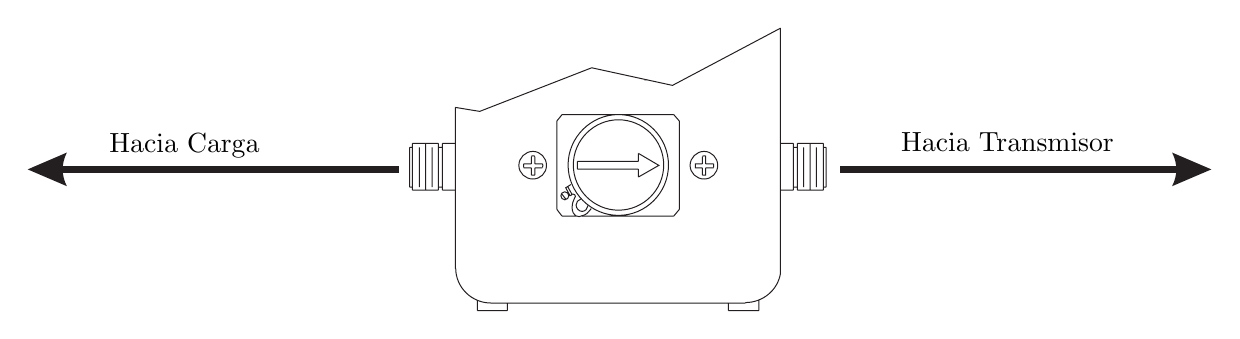
\begin{tikzpicture}[y=1cm, x=1cm, yscale=\globalscale,xscale=\globalscale, every node/.append, inner sep=0pt, outer sep=0pt]
  \begin{scope}[cm={ 0.2646,-0.0,-0.0,0.2646,(-7.9477, 11.3299)}]
    \path[draw=c231f20,line cap=butt,line join=miter,line width=0.0126cm,miter limit=2.613,cm={ 1.3333,-0.0,-0.0,-1.3333,(0.0, -101.4062)}] (30.866, -44.0806) -- (35.446, -44.0806)(35.446, -44.0886) -- (35.446, -44.0886).. controls (35.762, -44.0886) and (36.029, -44.3116) .. (36.079, -44.6136)(30.233, -44.7076).. controls (30.233, -44.3616) and (30.521, -44.0806) .. (30.866, -44.0806)(34.157, -45.6436) -- (32.501, -45.6436)(34.157, -47.4726) -- (32.148, -47.4726)(34.157, -45.6436) -- (34.258, -45.7656)(34.258, -47.3566) -- (34.258, -45.7656)(32.054, -47.3566) -- (32.054, -45.7656)(34.258, -47.3566) -- (34.157, -47.4726)(32.148, -47.4726) -- (32.054, -47.3566)(30.622, -44.1316) -- (30.622, -43.9446)(31.162, -43.9446) -- (30.622, -43.9446)(31.162, -43.9446) -- (31.162, -44.0806)(35.143, -43.9446) -- (35.143, -44.0806)(35.143, -43.9446) -- (35.69, -43.9446)(35.69, -44.1316) -- (35.69, -43.9446)(30.226, -47.6016) -- (30.226, -44.7006)(36.079, -44.6426) -- (36.079, -49.0276)(36.079, -44.6136).. controls (36.079, -44.6286) and (36.079, -44.6356) .. (36.079, -44.6496)(30.866, -44.0806) -- (30.866, -44.0806)(34.063, -46.5646).. controls (34.063, -47.0616) and (33.66, -47.4726) .. (33.163, -47.4726).. controls (32.666, -47.4726) and (32.256, -47.0616) .. (32.256, -46.5646).. controls (32.256, -46.0686) and (32.666, -45.6576) .. (33.163, -45.6576).. controls (33.66, -45.6576) and (34.063, -46.0686) .. (34.063, -46.5646) -- cycle(32.422, -46.6296) -- (33.523, -46.6296)(32.422, -46.4926) -- (33.523, -46.4926)(33.523, -46.7736) -- (33.523, -46.6296)(32.422, -46.6296) -- (32.422, -46.4926)(33.523, -46.7736) -- (33.89, -46.5576) -- (33.523, -46.3486)(33.523, -46.4926) -- (33.523, -46.3486)(34.733, -46.5146) -- (34.877, -46.5146)(34.733, -46.5866) -- (34.877, -46.5866)(34.949, -46.5576).. controls (34.949, -46.6946) and (34.841, -46.8096) .. (34.704, -46.8096).. controls (34.567, -46.8096) and (34.452, -46.6946) .. (34.452, -46.5576).. controls (34.452, -46.4206) and (34.567, -46.3126) .. (34.704, -46.3126).. controls (34.841, -46.3126) and (34.949, -46.4206) .. (34.949, -46.5576) -- cycle(34.733, -46.5146) -- (34.733, -46.3846)(34.675, -46.5146) -- (34.675, -46.3846)(34.675, -46.3846).. controls (34.69, -46.3846) and (34.697, -46.3846) .. (34.711, -46.3846).. controls (34.718, -46.3846) and (34.733, -46.3846) .. (34.74, -46.3846)(34.733, -46.7166) -- (34.733, -46.5866)(34.538, -46.5866) -- (34.675, -46.5866)(34.538, -46.5146) -- (34.675, -46.5146)(34.546, -46.5866).. controls (34.546, -46.5796) and (34.546, -46.5646) .. (34.546, -46.5576).. controls (34.546, -46.5436) and (34.546, -46.5366) .. (34.546, -46.5216)(34.675, -46.7166) -- (34.675, -46.5866)(34.74, -46.7236).. controls (34.733, -46.7306) and (34.718, -46.7306) .. (34.711, -46.7306).. controls (34.697, -46.7306) and (34.69, -46.7306) .. (34.675, -46.7236)(34.877, -46.5216).. controls (34.877, -46.5286) and (34.877, -46.5436) .. (34.877, -46.5576).. controls (34.877, -46.5646) and (34.877, -46.5796) .. (34.877, -46.5866)(31.658, -46.5146) -- (31.795, -46.5146)(31.658, -46.5866) -- (31.795, -46.5866)(31.867, -46.5576).. controls (31.867, -46.6946) and (31.759, -46.8096) .. (31.622, -46.8096).. controls (31.486, -46.8096) and (31.37, -46.6946) .. (31.37, -46.5576).. controls (31.37, -46.4206) and (31.486, -46.3126) .. (31.622, -46.3126).. controls (31.759, -46.3126) and (31.867, -46.4206) .. (31.867, -46.5576) -- cycle(31.658, -46.5146) -- (31.658, -46.3846)(31.594, -46.5146) -- (31.594, -46.3846)(31.594, -46.3846).. controls (31.608, -46.3846) and (31.615, -46.3846) .. (31.63, -46.3846).. controls (31.637, -46.3846) and (31.644, -46.3846) .. (31.658, -46.3846)(31.658, -46.7166) -- (31.658, -46.5866)(31.457, -46.5866) -- (31.594, -46.5866)(31.457, -46.5146) -- (31.594, -46.5146)(31.457, -46.5866).. controls (31.457, -46.5796) and (31.457, -46.5646) .. (31.457, -46.5576).. controls (31.457, -46.5436) and (31.457, -46.5366) .. (31.457, -46.5216)(31.594, -46.7166) -- (31.594, -46.5866)(31.658, -46.7236).. controls (31.651, -46.7306) and (31.637, -46.7306) .. (31.63, -46.7306).. controls (31.615, -46.7306) and (31.608, -46.7306) .. (31.594, -46.7236)(31.795, -46.5216).. controls (31.802, -46.5366) and (31.802, -46.5436) .. (31.802, -46.5576).. controls (31.802, -46.5646) and (31.802, -46.5796) .. (31.795, -46.5866);



    \path[draw=c231f20,line cap=butt,line join=miter,line width=0.0126cm,miter limit=2.613,cm={ 1.3333,-0.0,-0.0,-1.3333,(0.0, -101.4062)}] (33.977, -46.5646).. controls (33.977, -47.0116) and (33.61, -47.3786) .. (33.163, -47.3786).. controls (32.717, -47.3786) and (32.35, -47.0116) .. (32.35, -46.5646).. controls (32.35, -46.1186) and (32.717, -45.7516) .. (33.163, -45.7516).. controls (33.61, -45.7516) and (33.977, -46.1186) .. (33.977, -46.5646) -- cycle(36.9, -46.1686) -- (36.9, -46.8816)(36.727, -46.8816) -- (36.727, -46.1686)(36.497, -46.8816) -- (36.497, -46.1686)(36.382, -46.1116) -- (36.382, -46.9536)(36.31, -46.1116) -- (36.31, -46.9536)(36.85, -46.1116) -- (36.85, -46.9536)(36.612, -46.9536) -- (36.612, -46.1116)(36.85, -46.1116) -- (36.382, -46.1116)(36.31, -46.1686) -- (36.382, -46.1686)(36.31, -46.1116) -- (36.072, -46.1116)(36.85, -46.1686) -- (36.9, -46.1686)(36.85, -46.9536) -- (36.382, -46.9536)(36.31, -46.8816) -- (36.382, -46.8816)(36.31, -46.9536) -- (36.072, -46.9536)(36.85, -46.8816) -- (36.9, -46.8816)(29.578, -46.8816) -- (29.578, -46.1686)(29.808, -46.8816) -- (29.808, -46.1686)(29.405, -46.1686) -- (29.405, -46.8816)(29.693, -46.9536) -- (29.693, -46.1116)(29.923, -46.1116) -- (29.923, -46.9536)(29.995, -46.1116) -- (29.995, -46.9536)(29.455, -46.1116) -- (29.455, -46.9536)(29.455, -46.1116) -- (29.923, -46.1116)(29.455, -46.1686) -- (29.405, -46.1686)(29.995, -46.1116) -- (30.233, -46.1116)(29.995, -46.1686) -- (29.923, -46.1686)(29.455, -46.9536) -- (29.923, -46.9536)(29.455, -46.8816) -- (29.405, -46.8816)(29.995, -46.9536) -- (30.233, -46.9536)(29.995, -46.8816) -- (29.923, -46.8816)(32.22, -45.9456) -- (32.134, -46.0536)(32.27, -46.0106).. controls (32.27, -46.0466) and (32.234, -46.0826) .. (32.198, -46.0826).. controls (32.155, -46.0826) and (32.126, -46.0466) .. (32.126, -46.0106).. controls (32.126, -45.9746) and (32.155, -45.9386) .. (32.198, -45.9386).. controls (32.234, -45.9386) and (32.27, -45.9746) .. (32.27, -46.0106) -- cycle(32.386, -45.9966).. controls (32.371, -45.9676) and (32.357, -45.9316) .. (32.342, -45.8956).. controls (32.335, -45.8666) and (32.328, -45.8306) .. (32.328, -45.7946).. controls (32.328, -45.7656) and (32.335, -45.7296) .. (32.35, -45.7006).. controls (32.357, -45.6796) and (32.378, -45.6646) .. (32.393, -45.6506).. controls (32.407, -45.6436) and (32.429, -45.6366) .. (32.45, -45.6366) -- (32.458, -45.6366).. controls (32.494, -45.6436) and (32.522, -45.6506) .. (32.551, -45.6646).. controls (32.58, -45.6796) and (32.609, -45.7006) .. (32.63, -45.7296).. controls (32.652, -45.7446) and (32.666, -45.7656) .. (32.674, -45.7806)(32.386, -45.9966) -- (32.386, -46.0036).. controls (32.386, -46.0246) and (32.371, -46.0396) .. (32.35, -46.0396).. controls (32.342, -46.0396) and (32.335, -46.0396) .. (32.328, -46.0396)(32.306, -46.2126) -- (32.213, -46.1546) -- (32.292, -46.0106)(32.328, -46.0326) -- (32.292, -46.0106)(32.249, -46.1766) -- (32.328, -46.0326)(32.054, -45.7656) -- (32.148, -45.6436)(32.407, -45.6436) -- (32.148, -45.6436)(32.486, -45.9526).. controls (32.436, -45.9386) and (32.4, -45.8956) .. (32.4, -45.8446).. controls (32.4, -45.7876) and (32.45, -45.7296) .. (32.508, -45.7296).. controls (32.566, -45.7296) and (32.609, -45.7806) .. (32.616, -45.8376)(33.631, -48.0986) -- (33.689, -48.0986)(30.226, -47.6016) -- (30.665, -47.5296) -- (32.681, -48.3146) -- (34.135, -47.9976) -- (36.079, -49.0276);



    \path[draw=c231f20,line cap=butt,line join=miter,line width=0.0843cm,miter limit=2.613,cm={ 1.3333,-0.0,-0.0,-1.3333,(0.0, -101.4062)}] (29.21, -46.4856) -- (22.882, -46.4856);



    \path[fill=c231f20,even odd rule,cm={ 1.3333,-0.0,-0.0,-1.3333,(0.0, -101.4062)}] (22.529, -46.4856) -- (23.234, -46.1836).. controls (23.134, -46.3846) and (23.134, -46.5866) .. (23.234, -46.7886) -- (22.529, -46.4856);



    \path[draw=c231f20,line cap=butt,line join=miter,line width=0.0843cm,miter limit=2.613,cm={ 1.3333,-0.0,-0.0,-1.3333,(0.0, -101.4062)}] (37.152, -46.4856) -- (43.481, -46.4856);



    \path[fill=c231f20,even odd rule,cm={ 1.3333,-0.0,-0.0,-1.3333,(0.0, -101.4062)}] (43.834, -46.4856) -- (43.128, -46.7886).. controls (43.229, -46.5866) and (43.229, -46.3846) .. (43.128, -46.1836) -- (43.834, -46.4856);



    \node[anchor=south west] (text25) at (32, -39.15){Hacia Carga};



    \node[anchor=south west] (text1) at (51, -39){Hacia Transmisor};



  \end{scope}

\end{tikzpicture}

          \captionof{figure}{disposición para medición de potencia reflejada.}
          \label{fig:power_meas.reverse}
        \end{center}
        \end{minipage}
      \item Encender el transmisor y realizar la medición pulsando momentáneamente el botón de transmisión.
        \begin{equation*}
          P_r = *W
        \end{equation*}
        \begin{itemize}
          \item p/10 cm \quad Valor de la \( P_r \) (W) = 0.2
          \item p/13,7 cm \quad Valor de la \( P_r \) (W) = 0.3
          \item p/17 cm \quad Valor de la \( P_r \) (W) = 0.54
          \item p/32 cm \quad Valor de la \( P_r \) (W) = 2.4
        \end{itemize}
      \item Calcular el valor del ROE para cada uno de los irradiantes (31.70 cm, 17 cm, 16 cm y 13,5 cm.) por medio de
        su ecuación.

        Se define como relación de onda estacionaria a:
        \begin{equation}
          ROE = \frac{E_{MAX}}{E_{min}} = \frac{1 + \left| \Gamma \right|}{1 - \left| \Gamma \right|}
          \label{eq:roe}
        \end{equation}

        sabiendo que:
        \begin{equation}
          \Gamma = \sqrt{\frac{P_r}{P_i}}
          \label{eq:c_refl}
        \end{equation}

        reemplazando \ref{eq:c_refl} en \ref{eq:roe} nos queda:
        \begin{equation}
          ROE = \frac{\sqrt{P_i} + \sqrt{P_r}}{\sqrt{P_i} - \sqrt{P_r}}
        \end{equation}

        reemplazando los valores obtenidos, nos queda:
        \begin{equation*}
          ROE = *
        \end{equation*}
        \begin{itemize}
          \item p/10 cm \quad ROE = 1.6667
          \item p/13,7 cm \quad ROE = 2.2642
          \item p/17 cm \quad ROE = 3.1633
          \item p/32 cm \quad ROE = 3
        \end{itemize}
      \item Determinar cual de los irradiantes posee un menor ROE
      
        El elemento radiante de menor ROE es el que mide 10cm de longitud.
    \end{enumerate}
